\chapter{Results} \label{5: Results}

    This chapter compares different techniques used to optimise our deep learning model, as well as discussing reasons for these results. For the default classification task, where a loan is labelled either Fully Paid or Default, we refer to the Full Paid class as the negative class and Default as the positive class. As we are using highly imbalanced data, it would be simple to obtain high accuracy by simply predicting every data point as the majority class. Therefore, our results section will focus on three performance metrics, as defined by \cite{performance_metrics}:
    
    \begin{itemize}
      \item \textbf{Recall} (True positive rate): The performance of the minority (Default) class
        \begin{itemize}
            \item The proportion of Default instances that are correctly predicted as Default.
        \end{itemize}
      \item \textbf{Specificity} (True negative rate): The performance of the majority (Fully-Paid) class
        \begin{itemize}
            \item The proportion of Fully Paid instances that are correctly predicted as Fully Paid.
        \end{itemize}
      \item \textbf{AUC} (Area Under the Curve): The correctness of the classifier
        \begin{itemize}
            \item The proportion of correctly predicted instances.
            \item $AUC$ is $\frac{Recall + Specificity}{2}$ 
        \end{itemize}
    \end{itemize}
    
    The individual techniques discussed in this section were evaluated under the optimum model parameters, as listed in Section \ref{6: models}, except for the parameter under evaluation. The majority of the techniques and parameters chosen were based on previous academic work, and are referenced where applicable. In some instances, we used the academic publications to gauge appropriate value ranges and then performed a parameter search within space. All techniques were evaluated using 5-fold cross-validation. The magnitude of the dataset allowed us to split the data into large enough subsets such that the learning ability of our model would not be affected. 
    
    Table \ref{5: best_performance } shows the performance results under the optimum model parameters.
    
    \begin{table}[H]
        \centering
        \caption{Default Prediction Model Results} \vspace{0.5cm}
        \label{5: best_performance }
            \begin{tabular}{|p{6.5cm}|p{2.5cm}|p{2.5cm}|p{2.5cm}|}
                \hline \textbf{Model} & \textbf{Recall} & \textbf{Specificity} & \textbf{AUC} \\ \hline \hline
                Default Classification & 0.985 & 0.982  & 0.984 \\ \hline
            \end{tabular}
    \end{table}
    
    
    \section{Cost-Sensitive Learning ($\gamma$)}
        As discussed in Section \ref{class_imbalance}, we propose a weighted loss function with a Class Weight Scale-Factor ($\gamma$). A comparison of different $\gamma$ values can be seen in Table \ref{5: class_weight_scale_factor}.  
        
        \begin{table}[H]
            \centering
            \caption{Class Weight Scale-Factor ($\gamma$) Comparison Results} \vspace{0.5cm}
            \label{5: class_weight_scale_factor}
                \begin{tabular}{|p{6.5cm}|p{2.5cm}|p{2.5cm}|p{2.5cm}|}
                    \hline \mathbf{$\gamma$} & \textbf{Recall} & \textbf{Specificity} & \textbf{AUC} \\ \hline \hline
                    0.700 & 0.000 & 1.000 & 0.500 \\ \hline
                    0.800 & 0.300 & 1.000 & 0.650 \\ \hline
                    0.900 & 0.760 & 0.997 & 0.879 \\ \hline
                    1.000 & \textbf{0.985} & \textbf{0.982}  & \textbf{0.984} \\ \hline
                    1.100 & 0.993 & 0.800 & 0.897 \\ \hline
                    1.200 & 1.000 & 0.380 & 0.690 \\ \hline
                    1.300 & 1.000 & 0.000 & 0.500 \\ \hline
                \end{tabular}
        \end{table}
        
        The results in table \ref{5: class_weight_scale_factor} and graph in figure \ref{gamma_comparison} show there exists an apparent trade-off between Recall and Specificity. 
        
        \begin{figure}[H]
            \centering
            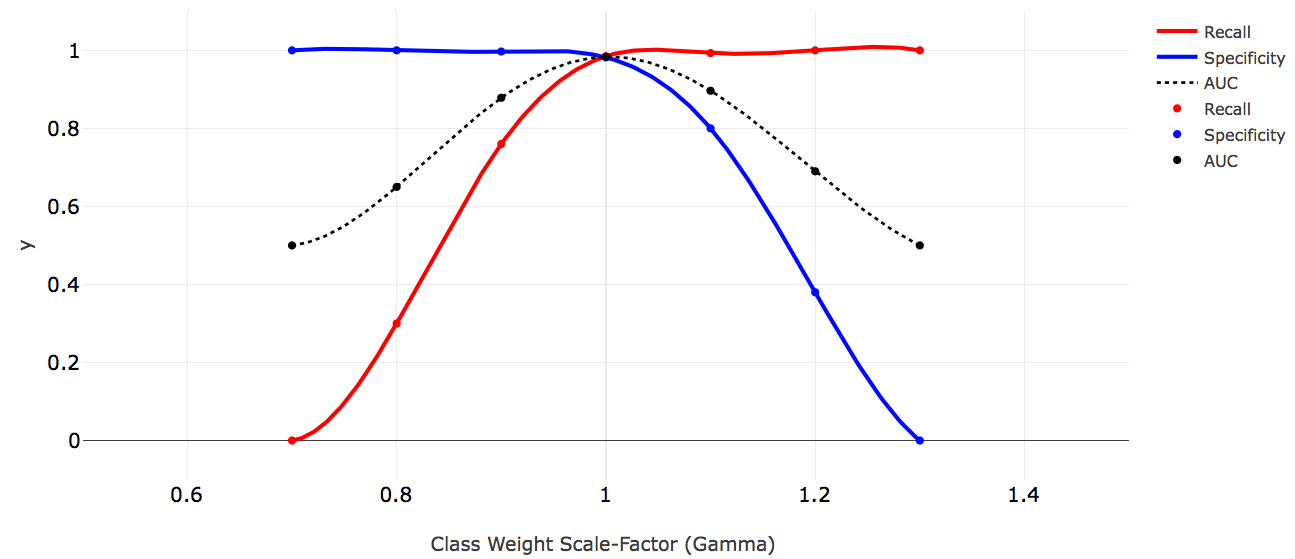
\includegraphics[width=0.99\textwidth]{Images/cost_sens_learn.png}
            \caption{A comparison between Recall, Specificity and AUC at different Class Weight Scale-Factor ($\gamma$) values.}
            \label{gamma_comparison}
        \end{figure}
        
        
        The optimum trade-off point between Recall, Specificity and AUC is where the lines in figure \ref{gamma_comparison} meet, at $\gamma$ = 1.0. A $\gamma$ value of 1 means that the loss function favours Recall and Specificity equally, irrespective of class ratios which have already been accounted for (as explained in \ref{class_imbalance}). Additionally, as discussed in section \ref{loss_function}, the neural network updates its weights and biases by minimising the output of loss function during training. This process means that we would expect to find that the optimal AUC value at $\gamma$ = 1.0, which is confirmed by our findings in table \ref{5: class_weight_scale_factor}. 
        
        We believed it was important to explore the results of cost-sensitive learning. If we consider the real world implications of the model, we hypothesise that incorrect classification of a Default loan would lead to greater financial consequences than miss-classifying a Fully Paid loan. In this scenario, the appropriate $\gamma$ value would be selected in order to best optimise the objective. An example of an objective would be the valuing of a loan portfolio, where it may be beneficial increase Recall performance. However, as this research has no outside objective, we will simply focus on producing a model that outputs the optimal AUC value, which is at $\gamma$ = 1.0. 

        
    \section{Model Architecture} \label{result_model_arc}
        The neural network architecture plays an important role in its ability to learn highly non-linear relationships. As discussed in \ref{research_model_arc}, selecting the optimal model architecture is not obvious without some trial and error. 
        
        We use as a baseline a single-layered network which acts as a linear regression model. We compare the architecture from \cite{mortgage_risk}, with a number of selected alternatives based on the research discussed in Section \ref{research_model_arc}. The results can be seen in table \ref{5: model_arc_comparison }.
        
        \begin{table}[H]
            \centering
            \caption{Model Architecture Comparison Results} \vspace{0.5cm}
            \label{5: model_arc_comparison }
                \begin{tabular}{|p{6.5cm}|p{2.5cm}|p{2.5cm}|p{2.5cm}|}
                    \hline \mathbf{Architecture} & \textbf{Recall} & \textbf{Specificity} & \textbf{AUC} \\ \hline \hline
                    133 : 2 (Linear) & 0.605 & 0.993  & 0.799 \\ \hline
                    133 : 100 : 2 & 0.961 & 0.957  & 0.959 \\ \hline
                    133 : 100:100 : 2 & \textbf{0.985} & \textbf{0.982}  & \textbf{0.984} \\ \hline
                    133 : 100:100:100:100:100 : 2 & 0.953 & 0.912  & 0.933 \\ \hline
                    133 : 200 : 2 \footnotemark[\getrefnumber{footnote_mortgage_risk}] & 0.954 & 0.851  & 0.953 \\ \hline
                    133 : 200:140 : 2 \footnotemark[\getrefnumber{footnote_mortgage_risk}] & 0.961 & 0.971  & 0.966 \\ \hline
                    133 : 200:140:140:140:140 : 2 \footnotemark[\getrefnumber{footnote_mortgage_risk}] & 0.951 & 0.899  & 0.920 \\ \hline

                \end{tabular}
                
            \vspace*{0.4cm}

            {\footnotesize Where, Architecture = \textbf{Input Layer : (Hidden Layer:)$^i$ : Output layer}}
        \end{table}
        
        \stepcounter{footnote}\footnotetext{From \cite{mortgage_risk} \label{footnote_mortgage_risk}}
        
        We found that the optimum architecture, given the $Default \, Prediction \, Objective$, consists of 2 hidden layers each with 100 nodes. Across all architectures, we found that two hidden layers perform better than both one and five hidden layers. The performance of the linear model is dominated by every other architecture with at least one hidden layer. The linear model has the lowest AUC and Recall values which indicate there exist complex non-linear relationships in the data that cannot be separated using linear regression. These results also suggest that adding multiple hidden layers allows the model to learn more complex non-linear relationships, directly resulting in higher predictive power and performance. We hypothesis that in order to obtain a better result, using a higher number of hidden layers, we should decrease the learning rate and increase the number of epochs during training, as recommended by \cite{shallow_vs_deep}. However, due to time restriction, based on the fact that the model takes over eight hours to train, we did not test this hypothesis. 
        
        
        % We hypothesis that adding more than 2 hidden layers ...?

    
    \section{Resampling}
        Resampling methods allow for repeated sampling of the original data to build new sample distribution. There are two main types of resampling; under-sampling and over-sampling. Resampling methods can be beneficial when handling imbalanced data, the work by \cite{imbalance_methods_3} concludes that "both over-sampling the minority class and down-sizing the majority class are very effective methods of dealing with the problem."
        
        \subsubsection{Random Under-Sampling vs SMOTE (1\% subset)} \label{SMOTE_exp}

        We have chosen to compare random under-sampling (Section \ref{under_sampling}( and SMOTE oversampling (Section \ref{SMOTE}). Due to the computational complexity of the SMOTE algorithm, we first performed a comparison on a 1\% subset of the data to obtain its potential effectiveness. Note that, in order to prevent overfitting, cross-validation was performed before any re-sampling methods were applied. Additionally, the resampling methods were only applied to the training set and not the validation set.
        
        \begin{table}[H]
            \centering
            \caption{Resampling Techniques Comparison Results (1\% subset)} \vspace{0.5cm}
            \label{5: table_resampling_techniques_subset}
                \begin{tabular}{|p{5cm}|p{2.25cm}|p{1.75cm}|p{2cm}|p{2cm}|}
                    \hline \textbf{Technique / Class Ratio} &  \textbf{Dataset \%} & \textbf{Recall} & \textbf{Specificity} & \textbf{AUC} \\ \hline \hline
                    None / 0.01:99.9 & 100\% & 0.359 & 0.955 & 0.657 \\ \hline
                    SMOTE / 15:85 & 130\% & 0.627 & 0.811  & 0.719 \\ \hline
                    SMOTE / 33:77 & 166\% & 0.659 & 0.730  & 0.693 \\ \hline
                    SMOTE / 50:50 & 200\% & 0.697 & 0.659  & 0.678 \\ \hline
                    Under-Sampling / 15:85 & 0.06\% & 0.797 & 0.740  & 0.769 \\ \hline
                    Under-Sampling / 33:77 & 0.03\% & 0.707 & 0.800  & 0.754 \\ \hline
                    Under-Sampling / 50:50 & 0.02\% & 0.567 & 0.845  & 0.706 \\ \hline
                \end{tabular}
        \end{table}
        
        The results in Table \ref{5: table_resampling_techniques_subset} show that SMOTE does not outperform random under-sampling. \cite{resamlping_methods} found that the SMOTE method increased the minority class recognition rate and sacrificed less overall clarification performance when compared to under-sampling methods, concluding that the main benefit of random oversampling is less information loss. However, we did not find this to be true on the 1\% subset. One explanation is that, after randomly under-sampling, the size of the dataset is still sufficiently large to be representative of the entire subset, and therefore information loss is much lower. Moreover, it is stated in the original literature that "the highest tested imbalanced training set was only about 10\%". Therefore, as the imbalance in our dataset is much more significant than 10\%, any comparison drawn between these two sets of results should be considerate of that fact. 
        
        \subsubsection{Random Under-Sampling} \label{random_under_sampling}
        The results in section \ref{SMOTE_exp} show that the SMOTE sampling method does not outperform under-sampling at any class ratio on a 1\% subset of the data. Given this, and that we estimate it would take significant computation time for the entire training dataset to be up-sampled using SMOTE, we decided to not compare this method further. We also noted that under-sampling is generally outperformed by SMOTE on smaller datasets. The fact that this did not occur in our comparison on a 1\% subset of the data means that we have more reason not to expect it to increase performance when applied to the entire dataset.   
        
        Nevertheless, we compared the under-sampling technique at different class ratios to see if our findings in Section \ref{SMOTE_exp} hold true when applied to the entire dataset. 

        \begin{table}[H]
            \centering
            \caption{Resampling Techniques Comparison Results} \vspace{0.5cm}
            \label{5: table_resampling_techniques}
                \begin{tabular}{|p{5cm}|p{2.25cm}|p{1.75cm}|p{2cm}|p{2cm}|}
                    \hline \textbf{Technique / Class Ratio} &  \textbf{Dataset \%} & \textbf{Recall} & \textbf{Specificity} & \textbf{AUC} \\ \hline \hline
                    None / 0.1:99.9 & 100\% & 0.413 & 0.991  & 0.702 \\ \hline
                    Under-Sampling / 15:85 & 0.06\% & \textbf{0.985} & \textbf{0.982}  & \textbf{0.984} \\ \hline
                    Under-Sampling / 33:77 & 0.03\% & 0.977 & 0.965  & 0.971 \\ \hline
                    Under-Sampling / 50:50 & 0.02\% & 0.971 & 0.966  & 0.685 \\ \hline
                \end{tabular}
        \end{table}
        
        From the result in table \ref{5: table_resampling_techniques} and \ref{5: table_resampling_techniques_subset}, we observed that both the SMOTE algorithm and under-sampling technique outperform our base case, where no re-sampling method is applied. We observe that when no resampling method is applied, irrespective of the weighted class ratios, the model performs poorly. We hypothesise that because the minority class instances are processed so infrequently, it makes the decision regions very small relative to the overall vector space and therefore it is difficult for the network to converge optimally. The low minority-to-majority class ratio means that the minority class is significantly underrepresented in the data. These findings agree with that by \cite{training_CNN}, which also found that the classifier performance is reduced when no re-sampling method is applied.    
        
        We also observe that classification performance, given the \textit{Default Prediction Objective}, decreases as the re-sample ratios become closer to 50:50. An explanation for this is that, if the training dataset is re-sampled at the 50:50 ratio, there now exists a large difference in the class ratios between the training data and the validation data. When this difference is large, the representation that the model is learning becomes less representative of the validation data, and therefore classification performance decreases. Additionally, in the case of under-sampling, as the class ratios become closer to 50:50, the total \% of the dataset being processed by the model decreases. This information loss could be another explanation for the decrease in classification performance.    
        
        Another consideration when analysing these results is that we are using a weighted loss function, discussed in section \ref{cost_sensitive_learning}, and data re-sampling. We can observe that the majority of published work has either focused on re-sampling techniques or weighted loss functions. However, recent publications in the medical industry have successfully combined these two techniques, see \cite{undersampling_CSL_medical}. We believe further research is required to support the effectiveness of combining both fully. 
    
    \section{Normalisation} \label{normalisation_results}
        Data Normalisation is an important data pre-processing step which enforces the integrity of the data by ensuring consistency across all the values. The normalisation techniques have chosen to compare are Min-Max, Z-Score and Decimal Point normalisation. 

       \vspace{20pt} \noindent We compare the different normalisation techniques in Table \ref{5: german_accuracy_scores_normalisation }.
    
            
        \begin{table}[H]
            \centering
            \caption{Normalisation Techniques Comparison Results} \vspace{0.5cm}
            \label{5: german_accuracy_scores_normalisation }
                \begin{tabular}{|p{6.5cm}|p{2.5cm}|p{2.5cm}|p{2.5cm}|}
                    \hline \textbf{Optimisation} & \textbf{Recall} & \textbf{Specificity} & \textbf{AUC} \\ \hline \hline
                    Baseline & 0.949 & 0.941 & 0.945 \\ \hline
                    Min-Max Normalisation \footnotemark[\getrefnumber{footnote_mortgage_risk}] & 0.970 & 0.959 & 0.965 \\ \hline
                    Z-Score Normalisation \footnotemark[\getrefnumber{footnote_mortgage_risk}] & 0.961 & 0.972 & 0.967 \\ \hline
                    Decimal Point Normalisation \footnotemark[\getrefnumber{footnote_mortgage_risk}] & \textbf{0.985} & \textbf{0.982}  & \textbf{0.984} \\ \hline
                \end{tabular}
        \end{table}
        % \unsure[inline]{CHECK THAT THE FOOTNOTE IN TABLE IS ON SAME PAGE £((@)£!@@@!}
        \stepcounter{footnote}\footnotetext{From \cite{normalisation_comparison} \label{footnote_normalisation}}

        

        
        From results in table \ref{5: german_accuracy_scores_normalisation }, we observe that applying a normalisation technique improves classification performance across every metric, in comparison to the baseline (no normalisation). We observe only a small difference between the three techniques compared in table \ref{5: german_accuracy_scores_normalisation }, with Decimal Point normalisation producing the highest classification performance. These results agree with the findings by \cite{normalisation_comparison}, where they compared the same three techniques, finding that Decimal Point outperforms both Min-Max and Z-Score Normalisation techniques with lower loss value and higher accuracy.
        
        Although the baseline model does not perform significantly worse than the other models with normalisation applied, if we remove the batch normalisation layer, performance decreases dramatically. This result highlights the importance of normalisation both, at the input level, and between layers, when training neural networks.  
        
    \section{Batch Normalisation, Dropout \& $L^2$ Regularisation} \label{BN_l2_drop_results}
        Batch Normalisation (BN) is an optimisation technique for improving stability and the performance of a neural network. In our implementation, we normalised the input data, as explained in section \ref{normalisation_results}. We apply batch normalisation after the activation functions between each layer; as explained in section \ref{batch_norm_sec}. Note that we do not need to use batch normalisation before the first layer as we provide the model with normalised data. 
        
        Dropout is a regularisation technique used to reduce overfitting. In our model, we applied dropout after each fully connected hidden layer and set the dropout probability to 0.5, as suggested by \cite{dropout_hinton}.
        
        $L^2$ Regularisation is another regularisation strategy, which achieves its objective by using a regularisation term, as discussed in Section \ref{l2_regularisation}. In our model, we apply $L^2$ Regularisation before each hidden layer using a regularisation term, $\lambda$, of 0.1; as suggested by \cite{l2_value}.  
        
        \begin{table}[H]
            \centering
            \caption{Batch Normalisation, Dropout \& $L^2$ Regularisation Comparison Results} \vspace{0.5cm}
            \label{5: table_overfitting_bn_dropout}
                \begin{tabular}{|p{6.5cm}|p{2.5cm}|p{2.5cm}|p{2.5cm}|}
                    \hline \textbf{Technique} & \textbf{Recall} & \textbf{Specificity} & \textbf{AUC} \\ \hline \hline
                    Baseline &0.911 & 0.798 & 0.855 \\ \hline
                    $L^2$ Reg & 0.891 & 0.928 & 0.909 \\ \hline
                    Dropout & 0.851 & 0.918 & 0.885 \\ \hline
                    Dropout \& $L^2$ Reg  & 0.850 & 0.908 & 0.879 \\ \hline
                    Batch Norm & 0.967 & 0.919 & 0.943 \\ \hline
                    Batch Norm \& $L^2$ Reg  & \textbf{0.985} & \textbf{0.982}  & \textbf{0.984} \\ \hline
                    Batch Norm \& Dropout & 0.0.947 & 0.929 & 0.938 \\ \hline
                    Batch Norm \& Dropout \& $L^2$ Reg  & 0.945 & 0.926 & 0.935 \\ \hline
                \end{tabular}
        \end{table}
        
        The results in table \ref{5: table_overfitting_bn_dropout} show that Batch Normalisation is an effective technique to improve classification performance. We observed that it outperformed dropout and that it was improved with the addition of $L^2$ Regularisation. We found that the need for dropout was strongly reduced when combined with batch normalisation. Additionally, we observed that all techniques showed improved performance over the baseline model. 
        
    % \section{Activation Functions ??}
    %             \unsure[inline]{Included in background so should i do a comparison?}



    % \section{Loss functions ??}
    %             \unsure[inline]{Included in background so should i do a comparison?}




    \section{Feature Selection}
        Feature selection is the process of selecting a subset of relevant features that provide the necessary information to train a model for a particular task. As discussed in Section \ref{sec: Feature_Engineering}, we have engineered a variety of novel features and removed redundant information, both of which should help to model in the classification task. 
        
        \subsection{With Monthly Performance Features} \label{monthly_performance_features_results}

            In this section, we will evaluate how the model performs under different subsets of features, using both the origination and monthly performance data to determine default prediction. We define the following subsets, using notation similar to that in Section \ref{formal_description}:  
        
            \begin{itemize}
              \item \textbf{Selection A}: Origination vector, $\textbf{O}$
              \item \textbf{Selection B}: Selection A and Monthly updates, $\textbf{M(t)}$
              \item \textbf{Selection C}: Selection B and Economic performance update vector, $\textbf{$\textbf{$\mathbf{E_{A}}$}$(t)}$
                \begin{itemize}
                    \item Where $\textbf{$\textbf{$\mathbf{E_{A}}$}$(t)}$ are features from \cite{mortgage_risk} as marked in Table \ref{4: table_economic_performance_features}.
                \end{itemize}
              \item \textbf{Selection D}: Selection C and Economic performance update vector, $\textbf{$\textbf{$\mathbf{E_{B}}$}$(t)}$
                \begin{itemize}
                    \item Where $\textbf{$\textbf{$\mathbf{E_{B}}$}$(t)}$ are novel features as shown in Table \ref{4: table_economic_performance_features} 
                \end{itemize}
            \end{itemize}
            
            \begin{table}[H]
                \centering
                \caption{Feature Selection Comparison Results (With Performance Updates)} \vspace{0.5cm}
                \label{5: table_feature_selection }
                    \begin{tabular}{|p{6.5cm}|p{2.5cm}|p{2.5cm}|p{2.5cm}|}
                        \hline \textbf{Feature Selection Type} & \textbf{Recall} & \textbf{Specificity} & \textbf{AUC} \\ \hline \hline
                        Feature Selection A & 0.690 & 0.724 & 0.707 \\ \hline
                        Feature Selection B & 0.862 & 0.925 & 0.893 \\ \hline
                        Feature Selection C & 0.973 & 0.952 & 0.963 \\ \hline
                        Feature Selection D & \textbf{0.985} & \textbf{0.982}  & \textbf{0.984} \\ \hline
                    \end{tabular}
            \end{table}
            
            From the results in table \ref{5: table_feature_selection }, we observe an improvement in classification performance as we increase the number of features through Selection [A-D]. 
            
            \subsubsection{Selection A}
            Selection A only considers a single data vector per loan, each containing information from the origination point. This constraint means that the sample selection size is much smaller than the others proposed, [B-D]. The classifier effectively acts as an indicator which could be used by the lenders at the time the loan is originally being considered to help evaluate a prospective mortgage buyer. The selection performs better than random\footnote{A random prediction model would, on average, result in Recall, Specificity and AUC score of 0.5.}, which suggests it is possible to predict the outcome of a loan given only the information directly provided by the mortgage vendor at origination.  
            
            \subsubsection{Selection B}
            Selection B resulted in the most significant increase in classification performance. After introducing the monthly performance vector, $\textbf{M(t)}$, each loan has, on average, 21 input vectors (i.e. the average duration of a loan). We hypothesise that it becomes easier for the model to determine the outcome of a loan as the age of the loans increase, resulting in a higher classification performance using Selection B over Selection A. We can validate this claim by examining the model's output on a sample of 50 default loans. We observe that on average, as the age of the loan increases, the output of the model moves closer to 1. This indicates that the model has a higher level of certainty, on average, as the loan age increases.  
            
            \subsubsection{Selection C}
            Selection C introduces the economic vector, $\textbf{$\textbf{$\mathbf{E_{A}}$}$(t)}$, as suggested by \cite{mortgage_risk}. This vector contains features in addition to what has been provided by the mortgage vendor in both the origination and monthly update vectors; discussed in detail in Section \ref{economic_update_features}. We observe a significant increase in classification performance across all three metrics when comparing Selection B and C. We deduce that the addition of geographically specific and time-based features does, in fact, improve overall performance. 
            
            \subsubsection{Selection D}
            Selection D introduces the economic vector, $\textbf{$\textbf{$\mathbf{E_{B}}$}$(t)}$. This vector contains features over and above what has been proposed by \cite{mortgage_risk}. We chose to extend the geographic-based features to both State and Zip-code, across multiple different metrics, as well as introduce additional economic data; discussed in detail in Section \ref{economic_update_features}. We again observed an increase in classification performance across all three metrics when comparing Selection C and D. We deduced that the addition of more geographically specific and time-based features did, in fact, further improve overall performance. We can see from figures \ref{fig:default_per_st_12_months} and \ref{fig:housing_price_index} in Section \ref{economic_update_features}, that these additional features can be used to help distinguish between 'Fully Paid' and 'Default' loans. We note that this observation does not guarantee that the performance of the model will improve; it is possible that the neural network using existing information already captures the observed separation between 'Fully Paid' and 'Default' on these features. However, this is likely not the case, as the results show an improvement in classification performance.

        \subsection{Without Monthly Performance Features}
        
            In this section, we will evaluate how the model performs under different subsets of features, using only origination data to determine Default prediction. i.e. For each Selection, we only have a single input vector per loan that was derived from data obtained at the origination date of the loan. We defined the following subsets, using notation similar to that in Section \ref{formal_description}:  
            
            \begin{itemize}
              \item \textbf{Selection A}: Origination vector, $\textbf{O}$
              \item \textbf{Selection A1}: Selection A and Economic performance update vector, $\textbf{$\textbf{$\mathbf{E_{A}}$}$(t)}$
              \begin{itemize}
                    \item Where $\textbf{$\textbf{$\mathbf{E_{A}}$}$(t)}$ are features from \cite{mortgage_risk} as marked in Table \ref{4: table_economic_performance_features}.
                \end{itemize}
              \item \textbf{Selection A2}: Selection A1 and Economic performance update vector, $\textbf{$\textbf{$\mathbf{E_{B}}$}$(t)}$
                \begin{itemize}
                    \item Where $\textbf{$\textbf{$\mathbf{E_{B}}$}$(t)}$ are novel features as shown in Table \ref{4: table_economic_performance_features} 
                \end{itemize}
    
            \end{itemize}
            
            \begin{table}[H]
                \centering
                \caption{Feature Selection Comparison Results (Origination Only)} \vspace{0.5cm}
                \label{5: table_feature_selection_origin }
                    \begin{tabular}{|p{6.5cm}|p{2.5cm}|p{2.5cm}|p{2.5cm}|}
                        \hline \textbf{Feature Selection Type} & \textbf{Recall} & \textbf{Specificity} & \textbf{AUC} \\ \hline \hline
                        Feature Selection A & 0.690 & 0.724 & 0.707 \\ \hline
                        Feature Selection A1 & 0.866 & 0.813 & 0.840 \\ \hline
                        Feature Selection A2 & 0.910 & 0.851 & 0.881 \\ \hline
                    \end{tabular}
            \end{table}
            
            From the results in table \ref{5: table_feature_selection }, we observed an improvement in classification performance as we increased the number of features through Selection [A-A2]. 
            
            \subsubsection{Selection A}
            Same as discussed in Section \ref{monthly_performance_features_results}.
            
            \subsubsection{Selection A1}
            Selection A1 introduces the economic vector, $\textbf{$\textbf{$\mathbf{E_{A}}$}$(t)}$, as suggested by \cite{mortgage_risk}. We observed an improvement in performance classification across all metrics when comparing Selection A1 with A. We concluded that the reason for this was the same as discussed for Selection C in Section \ref{monthly_performance_features_results}. 
            
            \subsubsection{Selection A2}
            Selection A2 introduces the economic vector, $\textbf{$\textbf{$\mathbf{E_{B}}$}$(t)}$. We observed an improvement in performance classification across all metrics when comparing Selection A2 with A1. We concluded that the reason for this is the same as discussed for Selection D in Section \ref{monthly_performance_features_results}. 
            
            It is interesting to note that the addition of $\textbf{$\textbf{$\mathbf{E_{A}}$}$(t)}$ and $\textbf{$\textbf{$\mathbf{E_{B}}$}$(t)}$ significantly improves classification performance at origination. This classification model could, in theory, be used by a mortgage vendor at the time the loan is originally being considered in order to help evaluate a prospective mortgage buyer
            
            
    
    
            

    
    \subsubsection{Conclusion}
        This section compared the results from a variety of methods; these include resampling, normalisation, regularisation and cost-sensitive learning. We also evaluated performance under different feature selections and model architectures, where all comparisons are evaluated using 5-fold cross-validation. The model achieved an AUC score of 0.984 under the optimum choice of parameters and techniques.


\clearpage

    
    